\documentclass[onecolumn,11pts]{IEEEtran}
\usepackage[utf8]{inputenc}
\usepackage{listings}
\usepackage{xcolor}
\usepackage{url}
\usepackage{hyperref}
\usepackage{graphicx}
\usepackage{anysize}
\usepackage[spanish]{babel}
\marginsize{3.5cm}{2.5cm}{3cm}{3cm} 
\hypersetup{
  colorlinks=false,       % false: boxed links; true: colored links
  pdfborder={0 0 0}       % remove ugly border from links
}


\markboth{Redes de Datos}%
{Informe}
\date{November 2016}

\begin{document}

\begin{titlepage}

\begin{center}
\vspace*{-1in}
\begin{figure}[htb]
\begin{center}

\includegraphics[scale=0.4]{UDP}
\end{center}
\end{figure}
Facultad de Ingeniería y Ciencias\\Escuela de Informática y Telecomunicaciones\\
\vspace*{0.15in}
\vspace*{1in}

\begin{LARGE}
\textbf{Laboratori N2: Redes de Datos \\ 'Cableado Estructurado'} \\
\end{LARGE}
\vspace*{1in}
\begin{large}
Profesor: José Pérez \\Ayudante: Alexis Inzunza \\ Fecha: 14-04-2017
\end{large}
\vspace*{0.3in}
\vspace*{1in}
\begin{large}
\begin{flushright}

Integrantes: \\
Benjamín Alvarez \\ Nicolás Reyes \\ 
\end{flushright}
\end{large}
\end{center}
\end{titlepage}


\tableofcontents % indice de contenidos

\cleardoublepage

\cleardoublepage

\title{Actividades de Laboratorio}

\maketitle

\section{Actividad: Contrucción de Cable (Directo y Cruzado)}

       La primera parte de este laboratorio consistió en armar dos cables de categoría 5, uno directo y uno cruzado, utilizando los materiales entregados y cumpliendo con las tablas de los diagramas de la especificación T568-A y T568-B que sustenta la construcción de dichos cables.
Pero primero debemos entender la diferencia entra ambos cables. El cable directo se puede identificar por la siguiente característica: En ambos extremos del cable se tiene las misma configuración, es decir, si elegimos, por ejemplo, la especificación T568-B, esta se deberá utilizar en ambos extremos. Mientras tanto, el cable cruzado deberá tener en cada extremo una especificación diferente.
Para hacer esto se nos fueron entregados 4 rosetas RJ45, dos trozos de cable de red y un alicate RJ45. También, debimos seguir ciertos pasos dados por el ayudante y escritos en el PDF de el Laboratorio.

       


        Tambien se nos fueron entregados una serie de pasos a seguir para que la confeccion del cable fuera mas fácil y rapida. Los pasos son los siguientes:

\begin{enumerate}
\item Quitar 5cm. de la envoltura de ambos extremos del cable, esto con tal de dejarlo descubierto y maniobrable.
\item Se organizan los pares de acuerdo a la norma que se utilizará.
\item Aplanar y enderezar los cables para ingresarlo en la roseta, siempre cuidando que la altura de estos quedara lo mas pareja posible.
\item Insertar los cables a la roseta, cuidando que todos lleguen hasta el final y que la envoltura quede dentro para proteger el cable.
\item En el alicate RJ45, insertar la roseta para crimpar el extremo, apretando fuertemente con ambas manos.
\item Realizar estos pasos nuevamente para el otro extremo del cable, teniendo en cuenta la norma que vas a usar (en el caso que sea directo o cruzado).
\item  Al tener el cable listo, el ayudante debe revisar su funcionamiento.
\end{enumerate}
\section{Cuestionario e Invesstigación}
\begin{enumerate}
    \item Describa brevemente las categorías existentes de cable UTP y sus usos: \\ -Categoría 1: Se utiliza principalmente para conexiones telefónicas. \\ -Categoría 2: Es capaz de transmitir datos hasta de 4 Mbps \\ -Categoría 3: Es un par trenzado sin blindar ,que puede alcanzar velocidades de hasta 10 Mbps. \\ -Categoria 4:Alcanza velocidades de 16 Mbps.Se utiliza sobre todo en las redes Token Ring. \\ -Categoría 5:Alcanza velocidades de 1000 Mbps.se utilizan para conexiones de computadoras conectadas a redes de área local. \\ -Categoría 5e: Es una mejora de la categoria 5, la principal mejora es que es más adecuado para ser utilizado con Gigabit Ethernet \\ -Categoría 6:En esta categoria se alcanzan velocidades de 1Gbps,una característica de este cable es que es compatible con versiones anteriores como la categoría 5e y categoría 3 \\ -Categoría 7:Alcanza 10Gbps y tiene un alcanze de hasta 100 metros, también es compatible con versiones  anteriores como la categoría 5 y la categoría \\  
    \item ¿Para qué situaciones debería usar un cable STP? Explique: \\ 
	Se utiliza cuando existe el riesgo de que se produzcan interferencias o ruidos 
            eléctricos, ya que en este cable cada par trenzado viene recubierto con una malla
            protectora que produce un efecto “pantalla” (a diferencia del cable UTP que solo
            presenta la cubierta de pvc). \\

\end{enumerate}
\section{Conclusión}
Al llevar la teoría a la práctica, vemos y conocemos las dificultades propias de realizar una conexión de tipo directa y una cruzada,  recordemos que la directa es aquella que tiene en ambos lados del cable la misma norma (en nuestro caso T568-A hacia T568-A). Mientras la cruzada es la que tiene tiene en cada extremo una norma diferente (T568-A y T568-B). Además nos dimos cuenta de la importancia de que cada cable llegue hasta el final de la roseta ya que si uno no llega puede ser que el cable siga funcionando pero  no estaría funcionado al 100 y la conexión podría presentar problemas a futuro.

\newpage

\section{Figuras}
\begin{figure}[h!]
\centering
 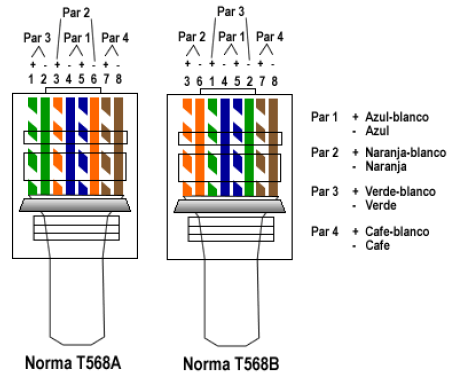
\includegraphics[scale=0.4]{Screenshot_2}
\caption{Normas de Cable T568-A Y T568-B}
\label{fig:Screenshot_2}
\end{figure}

\begin{figure}[h!]
\centering
 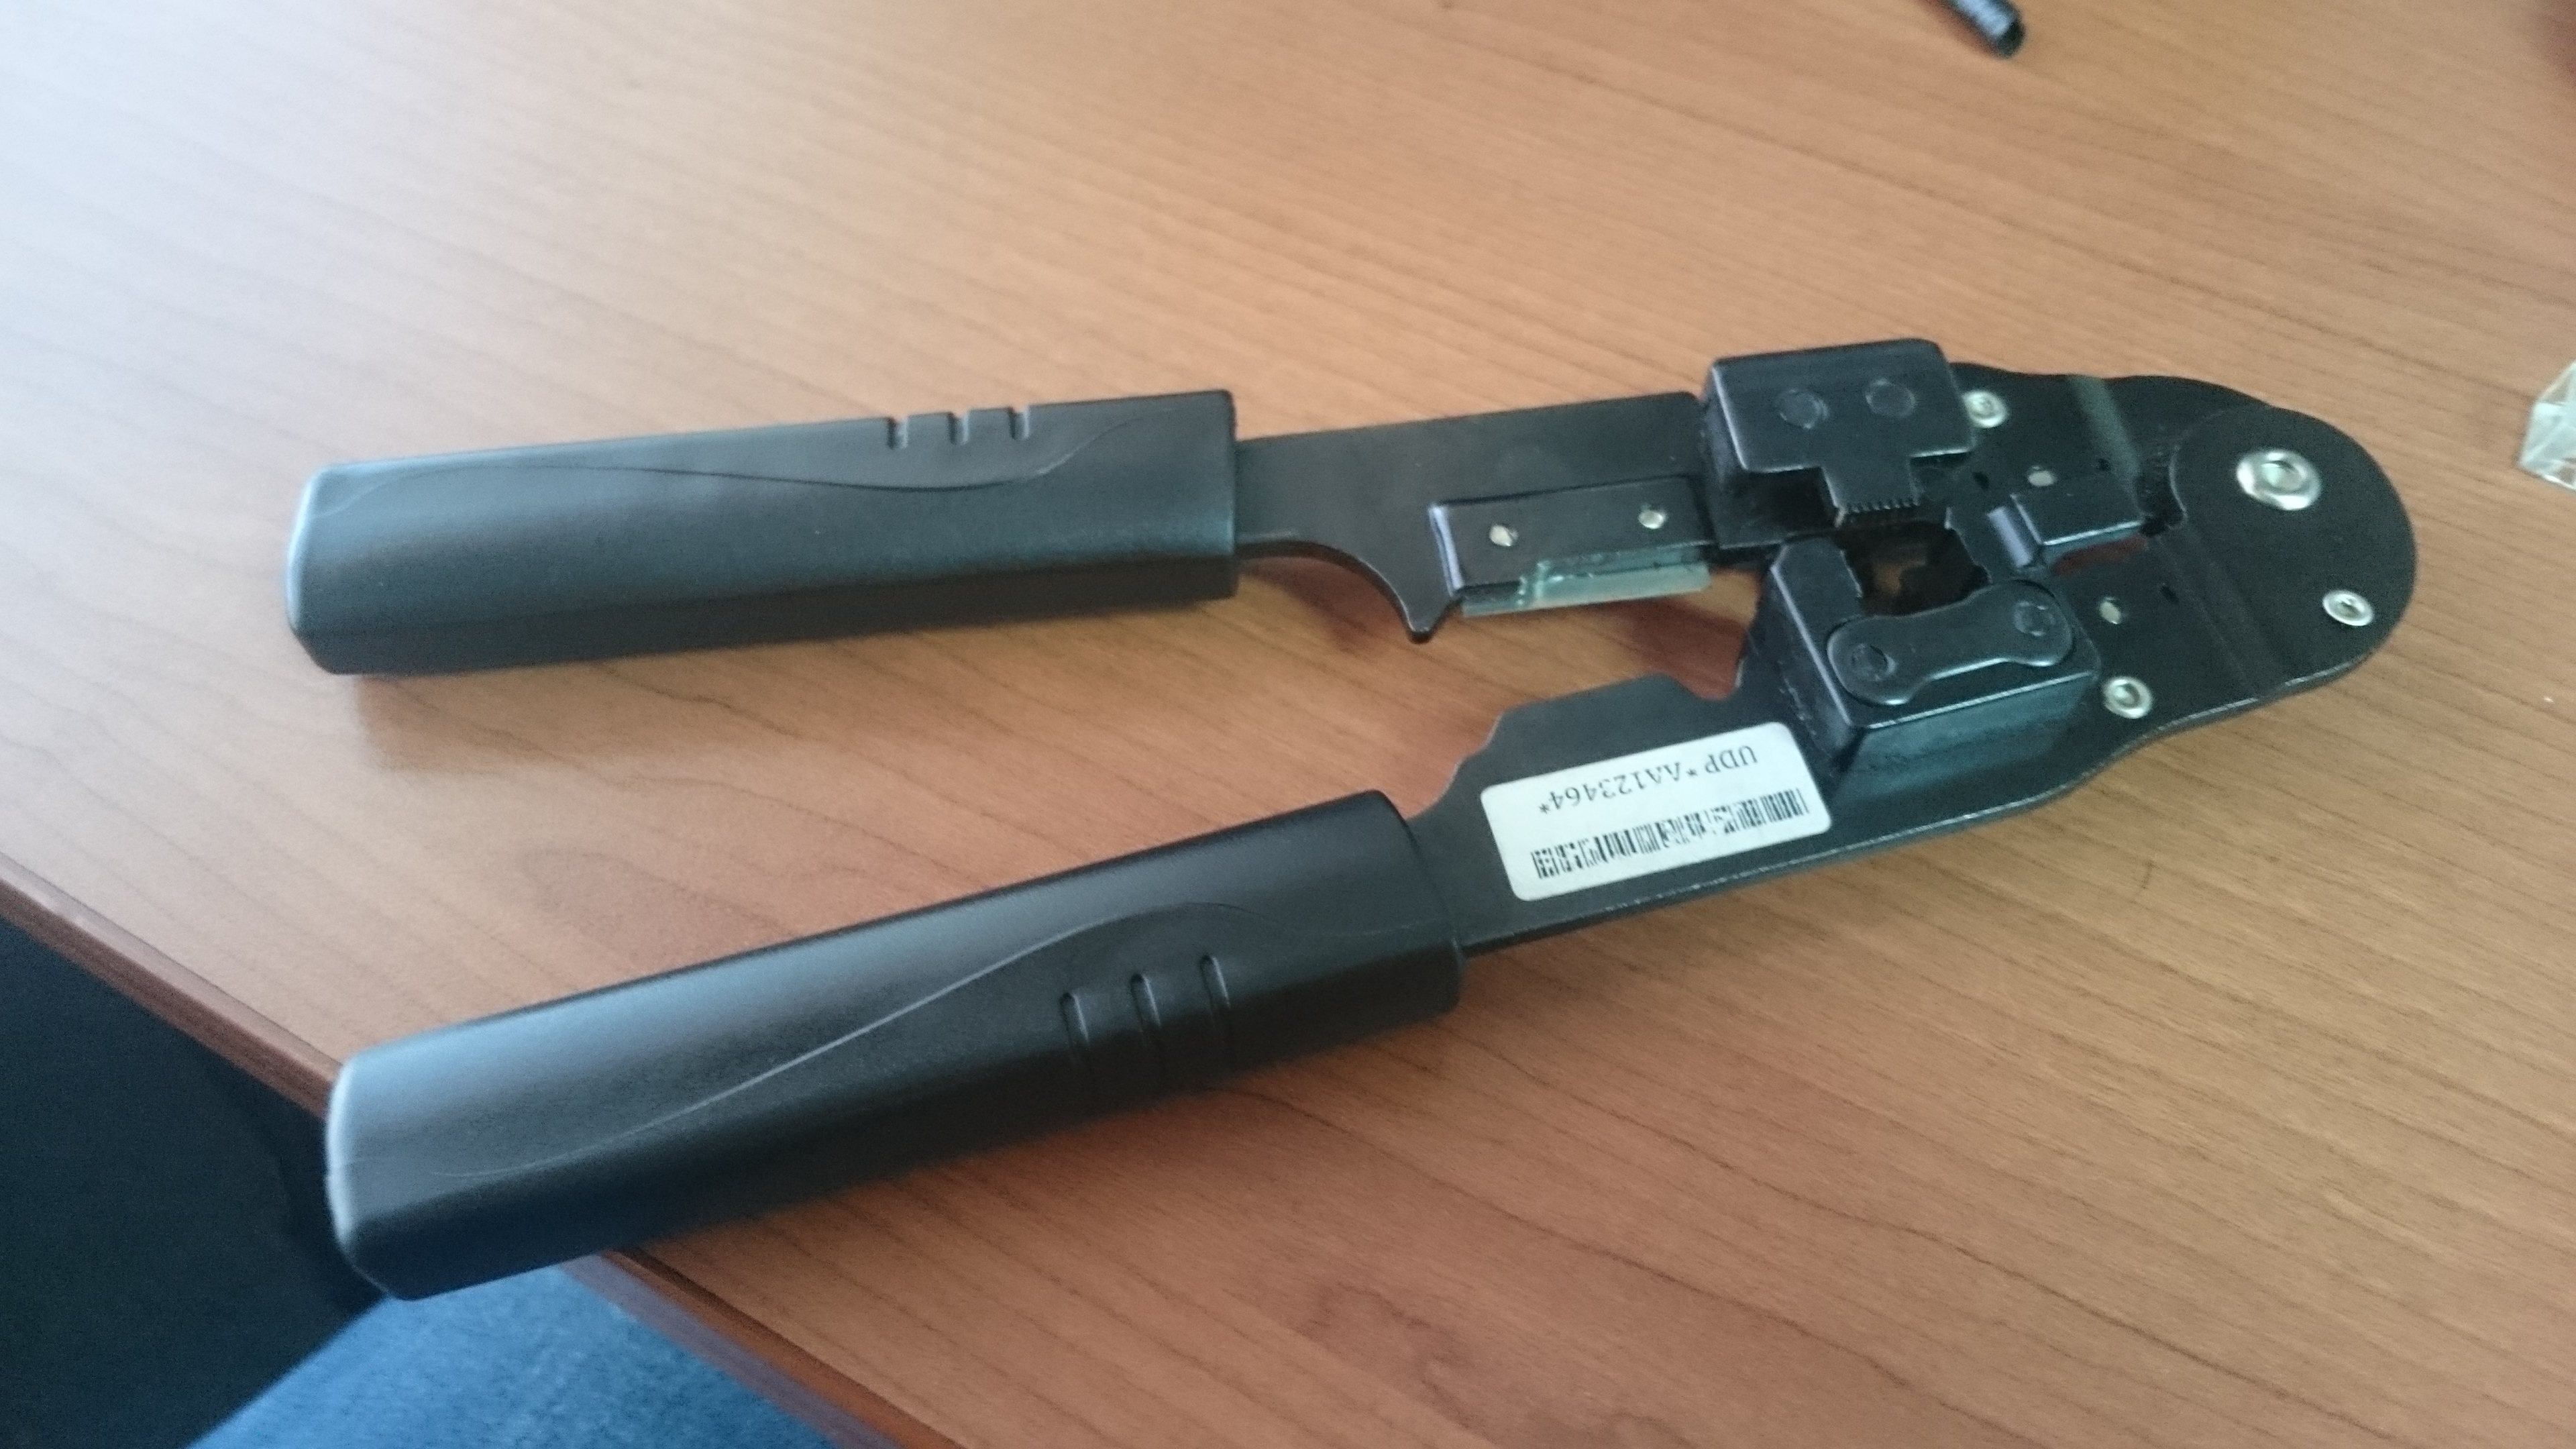
\includegraphics[scale=0.04]{DSC_0633}
\caption{Alicate RJ45}
\label{fig:DSC_0633}
\end{figure}

\begin{figure}[h!]
\centering
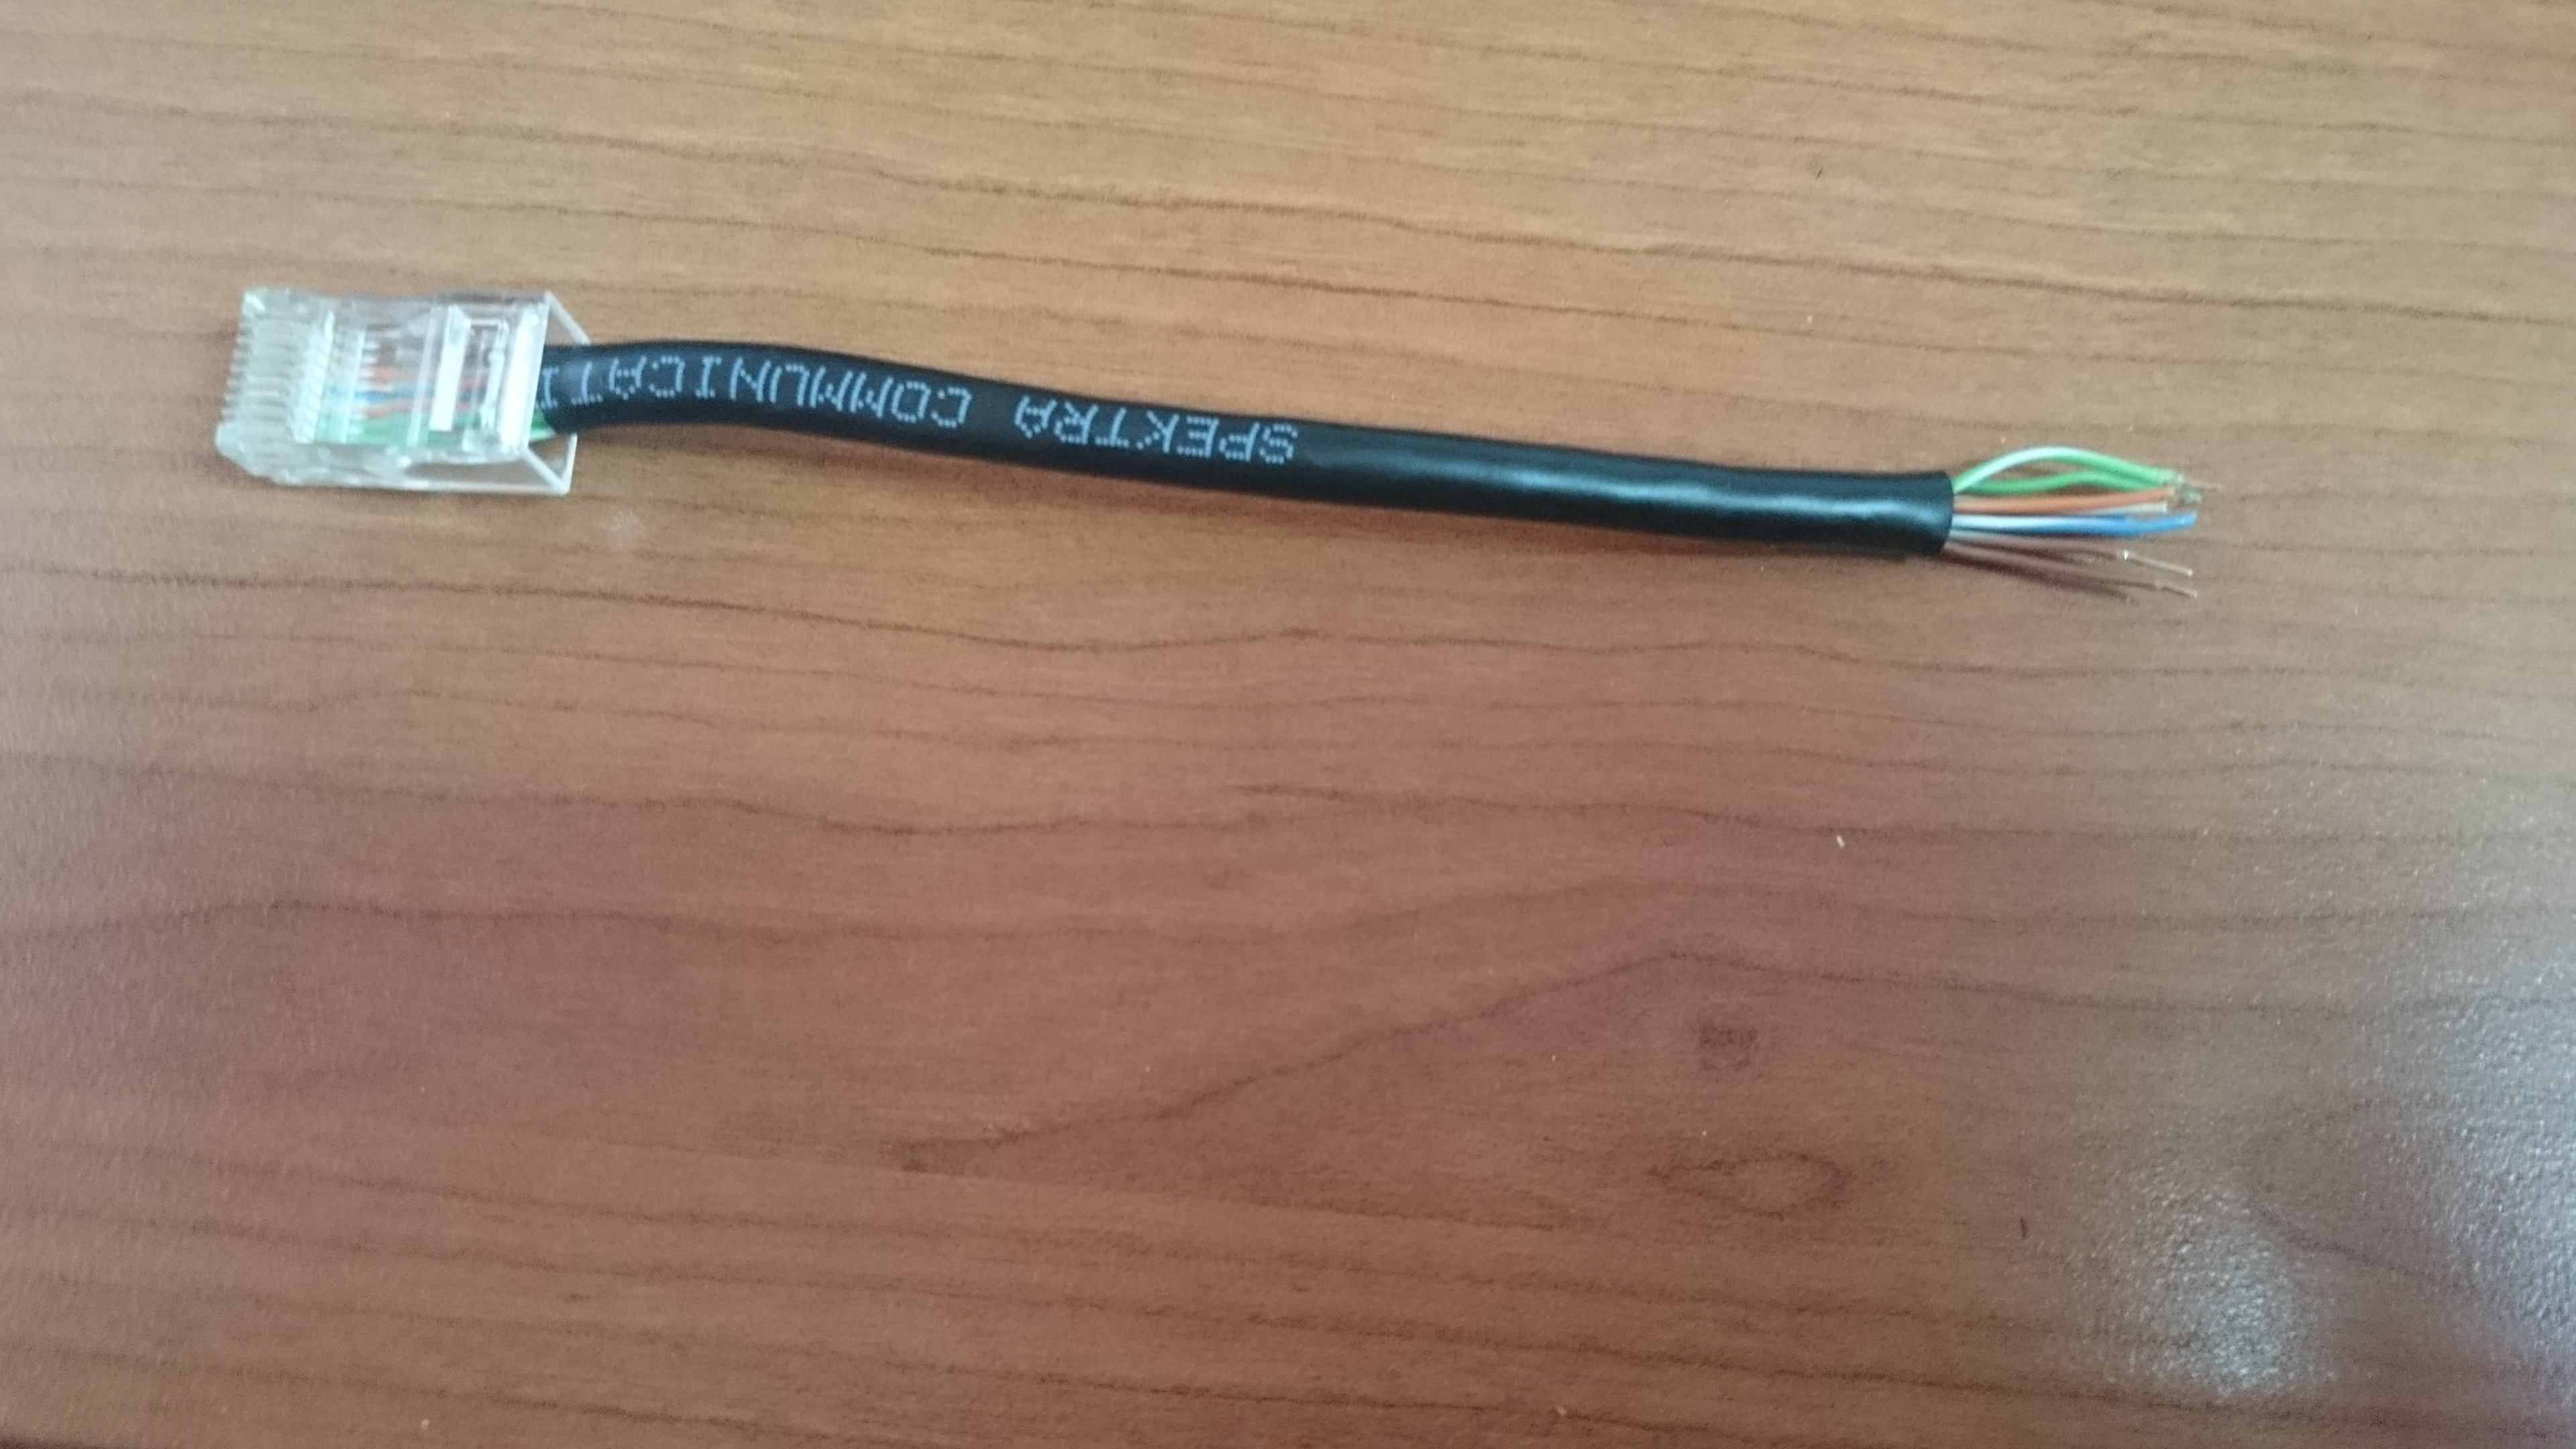
\includegraphics[scale=0.04]{DSC_0636}
\caption{Ordenando los cables antes de ingresarlos en la roseta}
\label{fig:DSC_0636}
\end{figure}



\begin{figure}[h!]
\centering
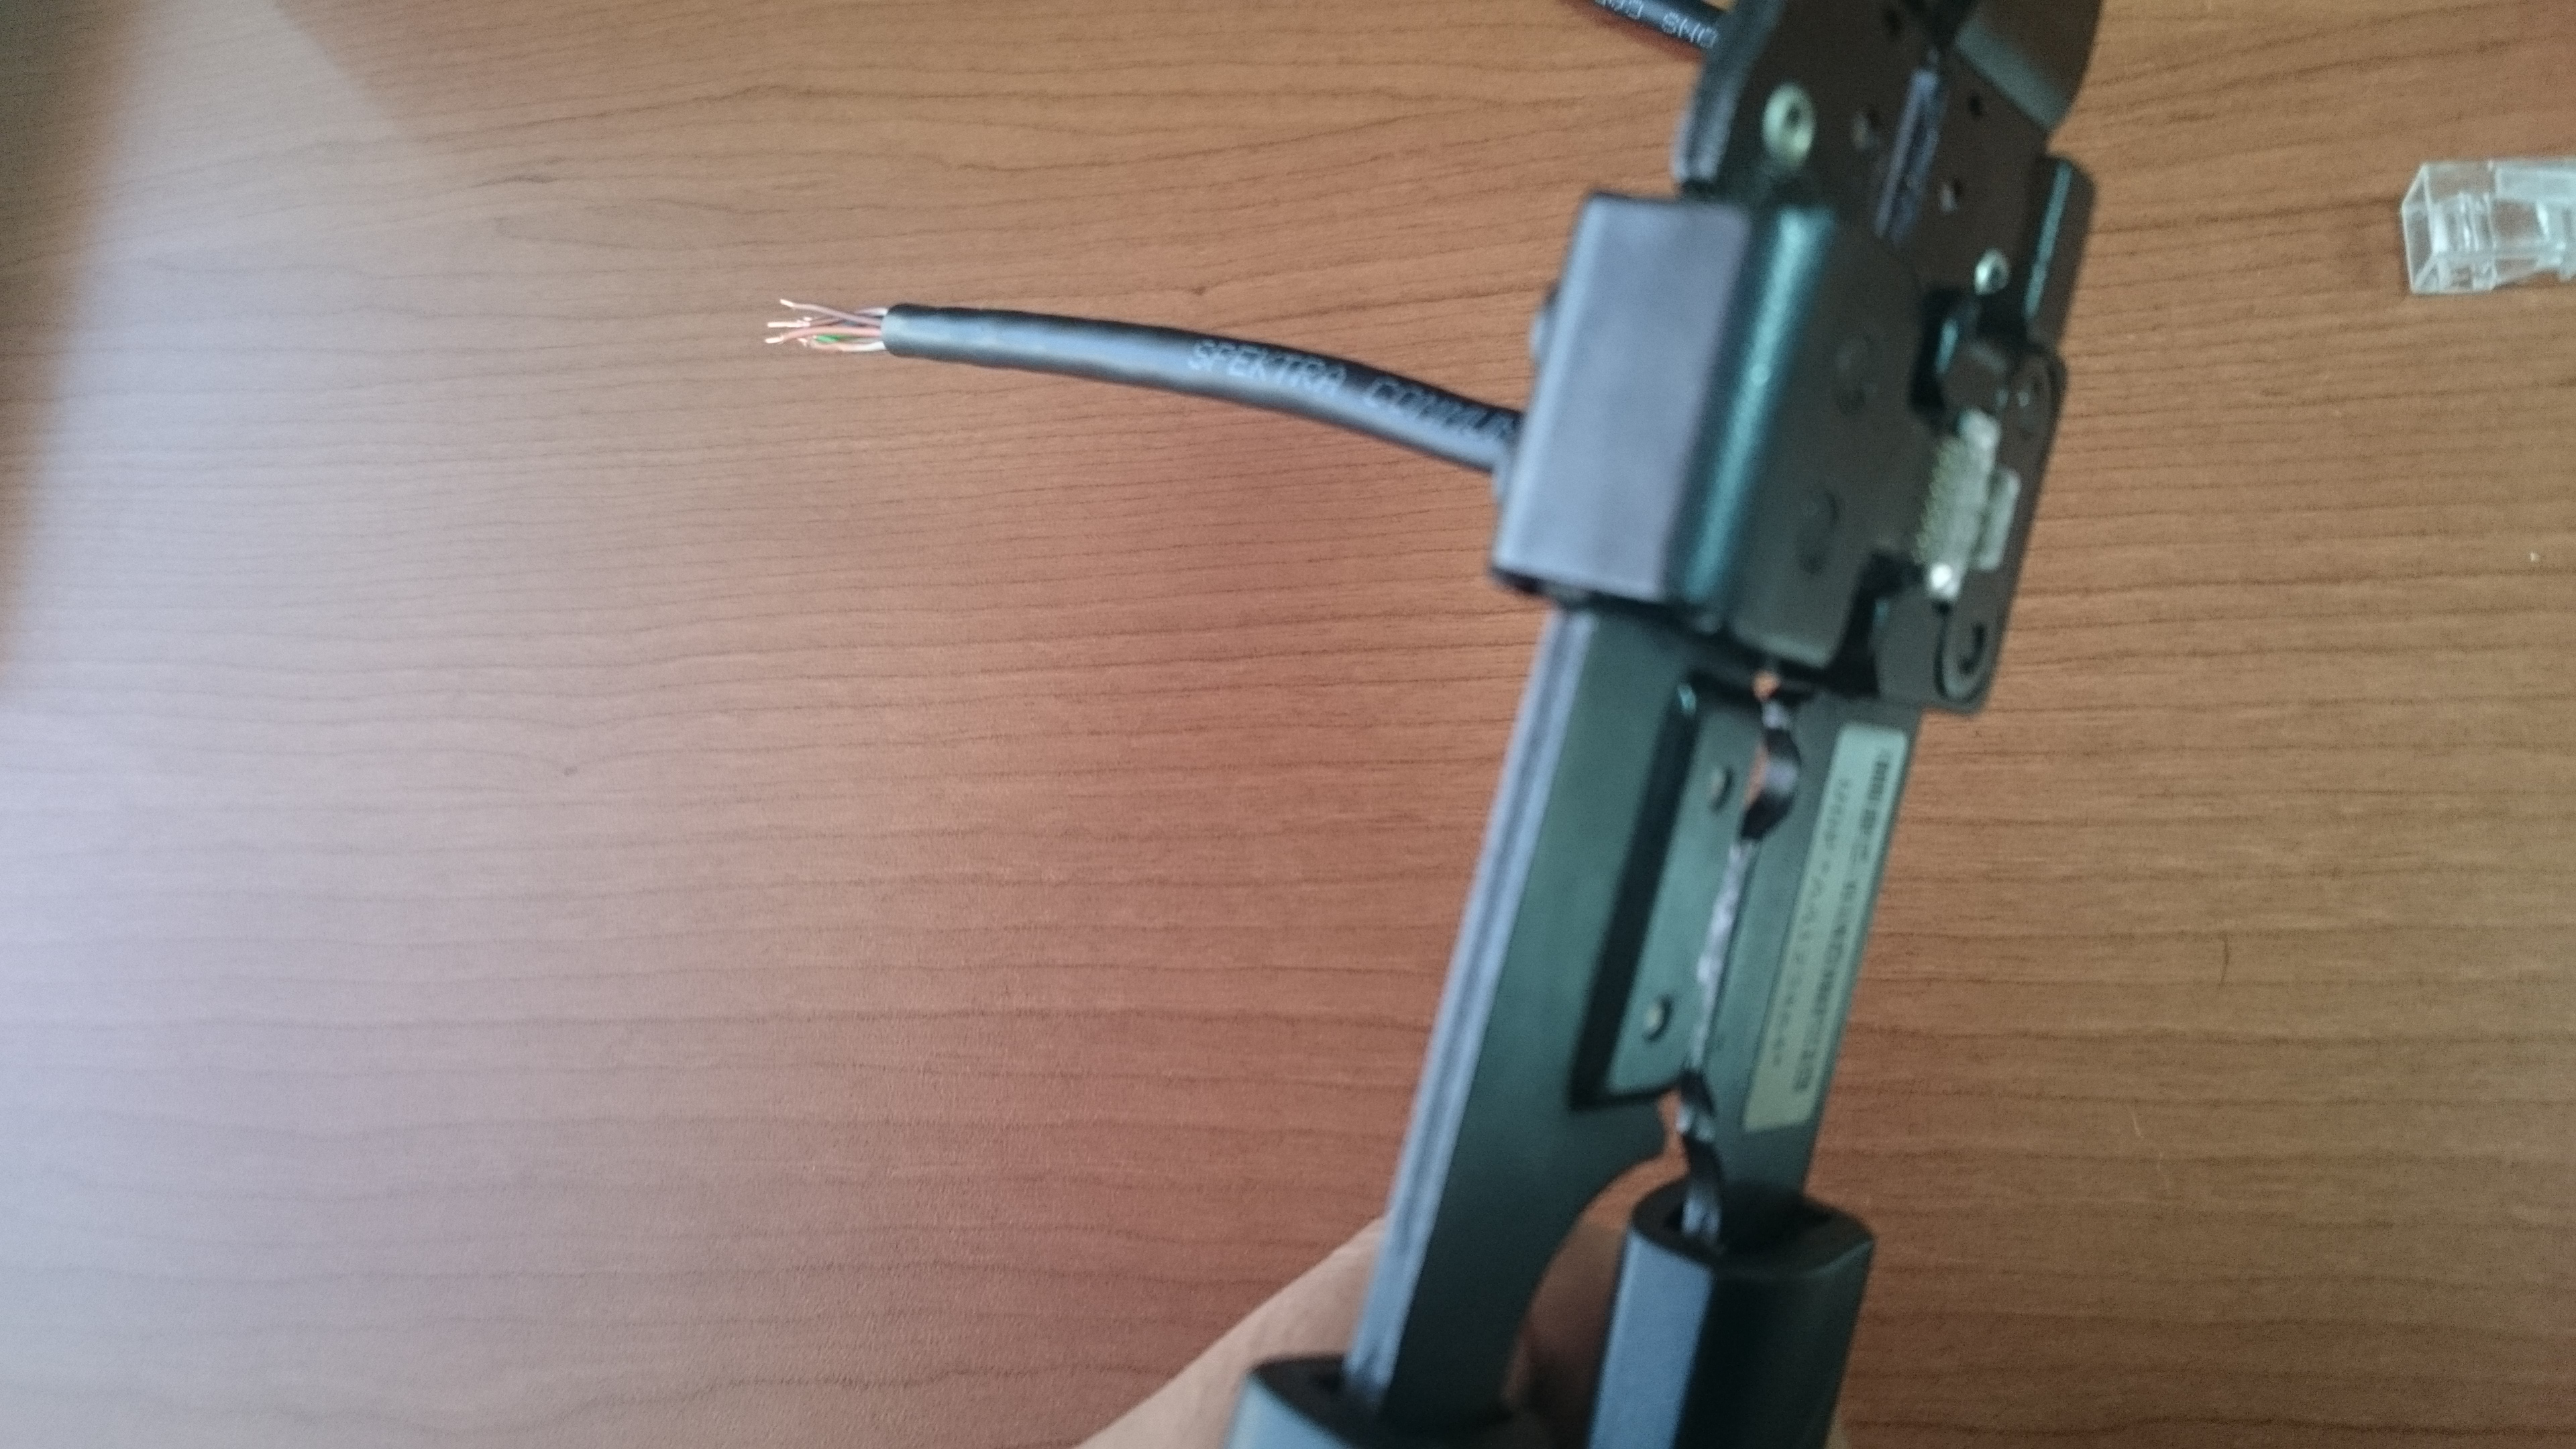
\includegraphics[scale=0.04]{DSC_0632}
\caption{Apretando RJ45 con el alicate}
\label{fig:DSC_0632}
\end{figure}

\begin{figure}[h!]
\centering
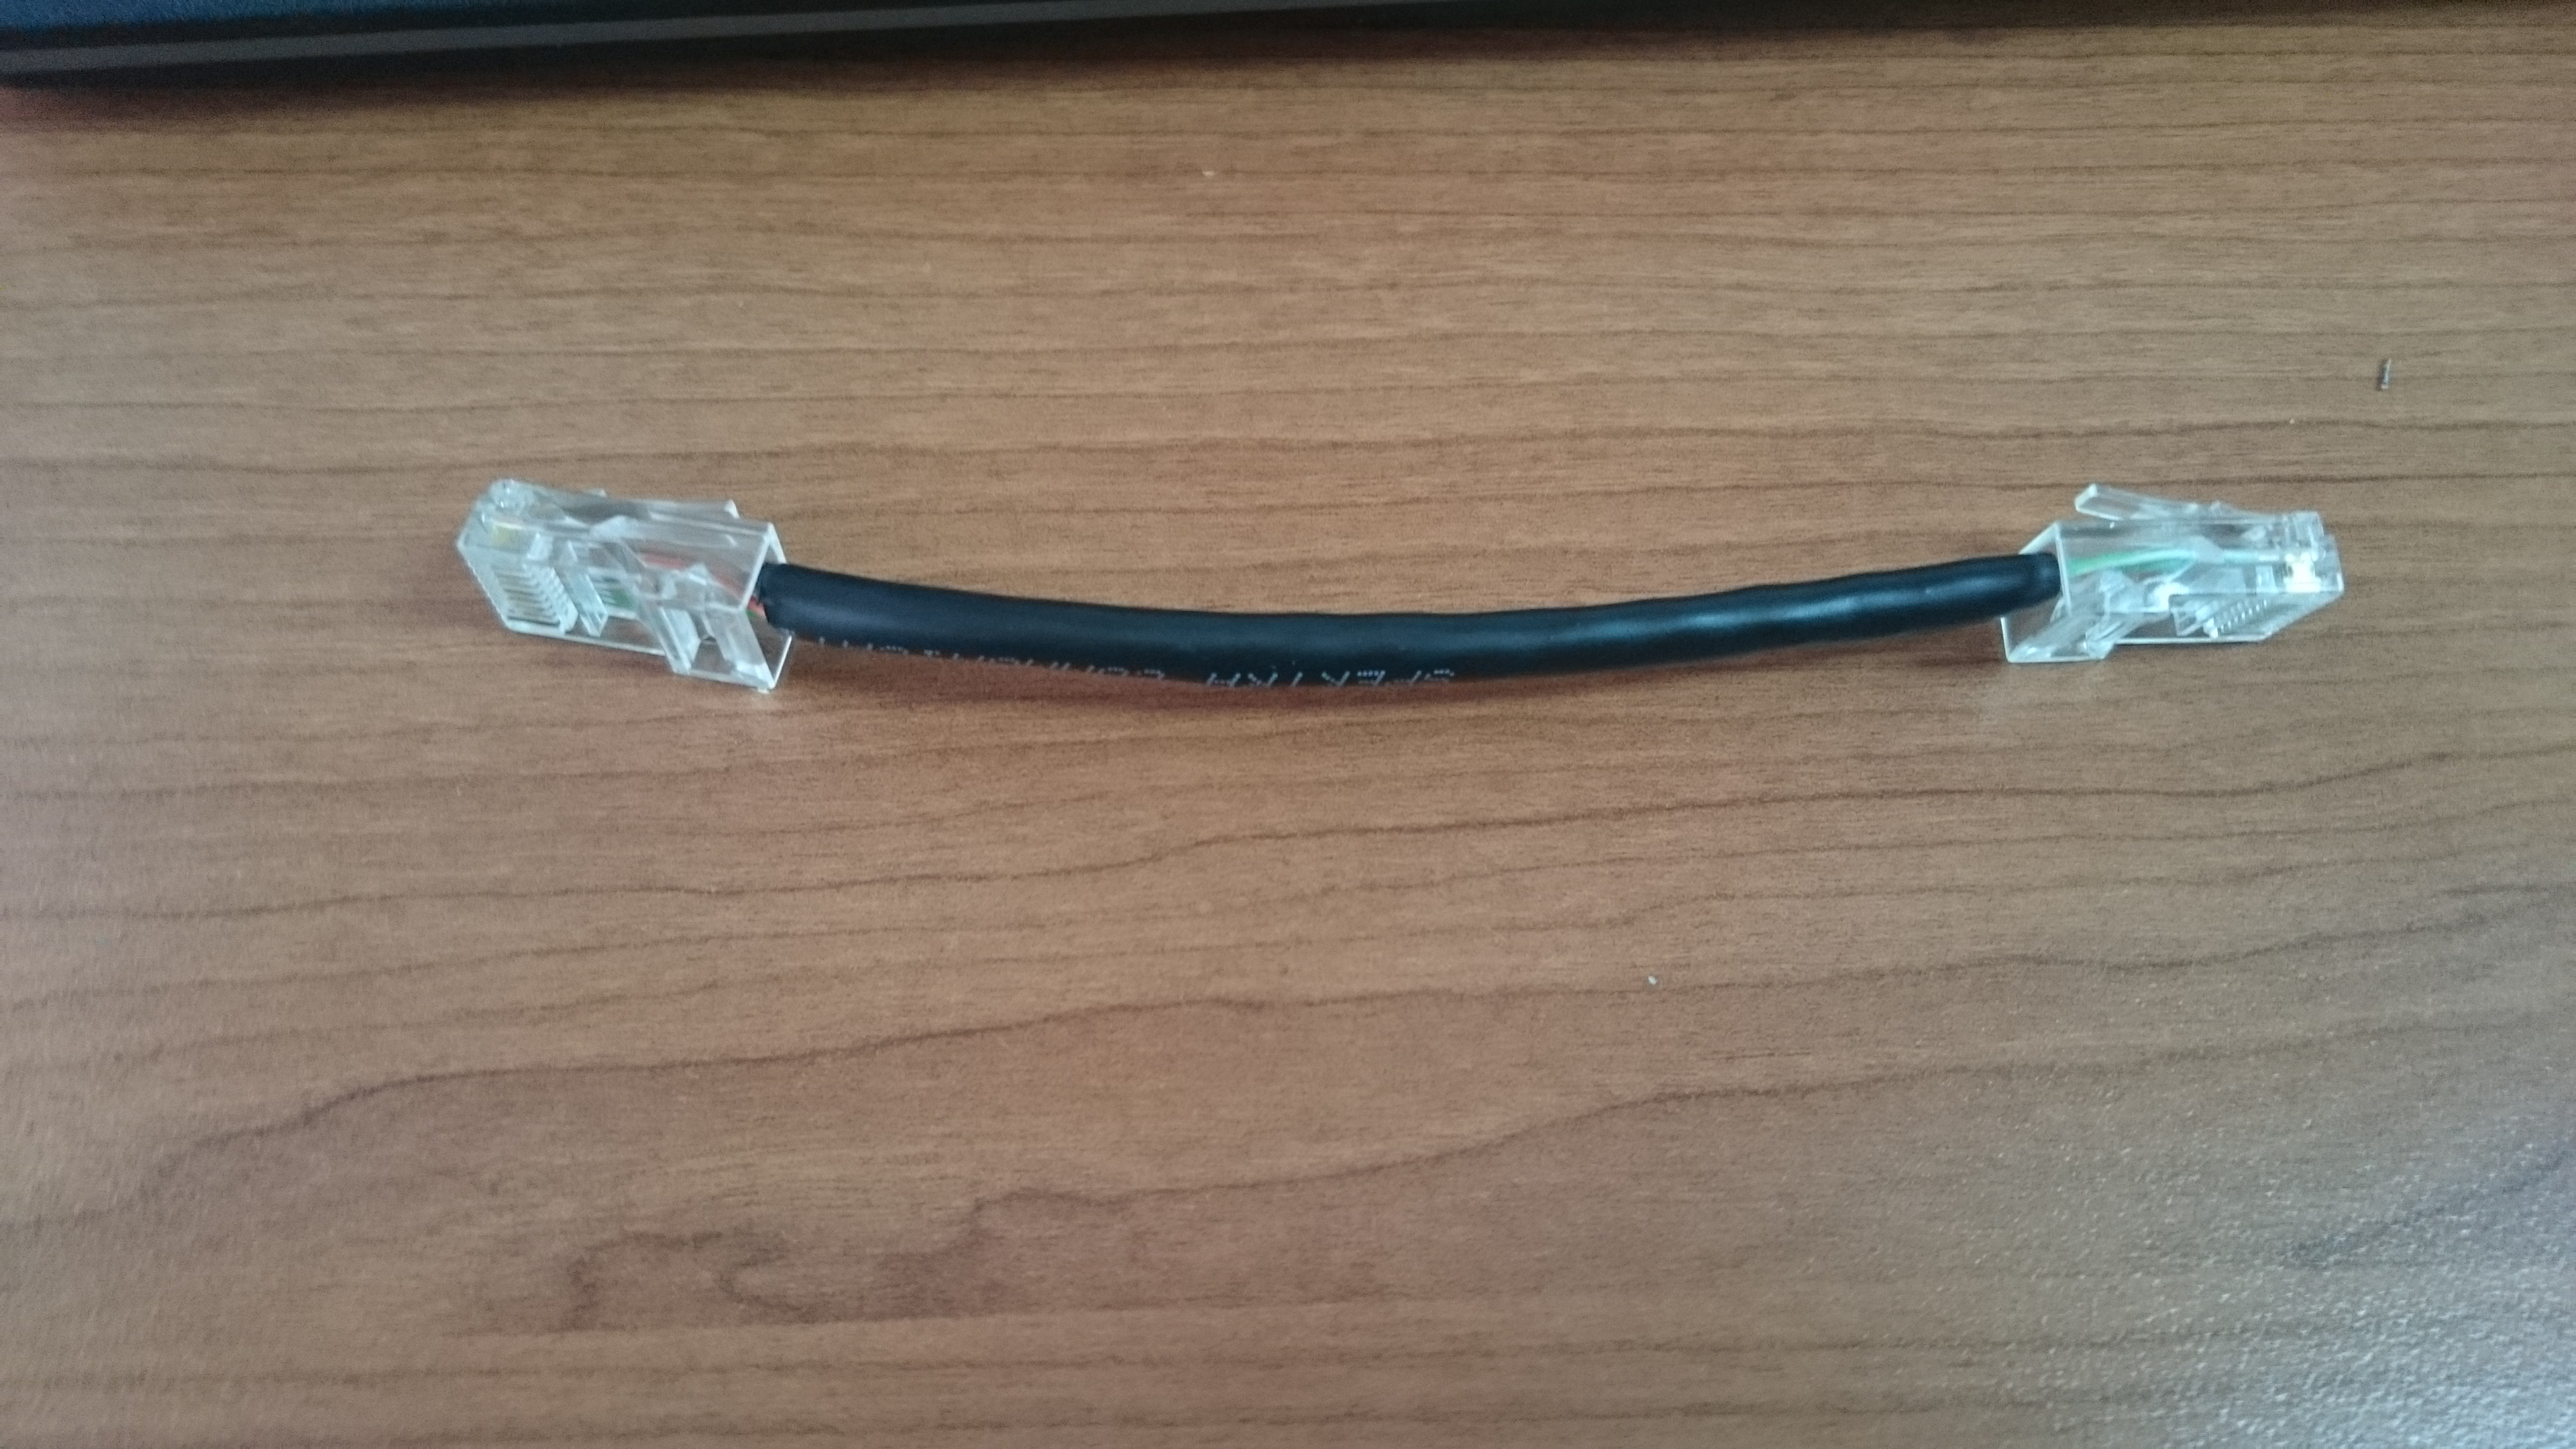
\includegraphics[scale=0.04]{DSC_0634}
\caption{Cable Directo Listo}
\label{fig:DSC_0634}
\end{figure}  



\clearpage

\begin{thebibliography}{15}

\bibitem{mfp}
  Cable de para Trenzado,
  \emph{Wikipedia}
  \url{https://es.wikipedia.org/wiki/Cable_de_par_trenzado#Categor.C3.ADas}
  

\end{thebibliography}

\end{document}